\documentclass[11pt,a4paper]{article}
\usepackage{tikz}
\usepackage{amsmath}
\usetikzlibrary{decorations.markings}
\usepackage{xcolor}

\begin{document}

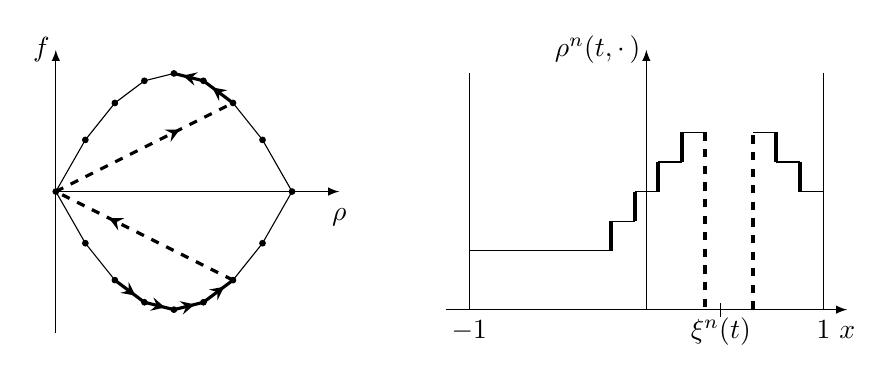
\begin{tikzpicture}[every node/.style={anchor=south west,inner sep=2pt}, x=30mm, y=60mm]

\draw[-latex] (0,0) -- (1.2,0) node[below] {\strut $\rho$};
\draw[-latex] (0,-.3) -- (0,.3) node[left] {\strut $f$};
\foreach \Point in {(0.,0.), (0.125,0.109375), (0.25,0.1875), (0.375,0.234375), (0.5,0.25), (0.625,0.234375), (0.75,0.1875), (0.875,0.109375), (1.,0.), (0.125,-0.109375), (0.25,-0.1875), (0.375,-0.234375), (0.5,-0.25), (0.625,-0.234375), (0.75,-0.1875), (0.875,-0.109375)}
    \draw[fill=black] \Point circle (1pt);

\begin{scope}[line width=0.4mm,decoration={markings, mark=at position 0.7 with {\arrow{stealth}}}]
\draw[postaction={decorate}] (0.25,-0.1875) -- (0.375,-0.234375);
\draw[postaction={decorate}] (0.375,-0.234375) -- (0.5,-0.25);
\draw[postaction={decorate}] (0.5,-0.25) -- (0.625,-0.234375);
\draw[postaction={decorate}] (0.625,-0.234375) -- (0.75,-0.1875);
\draw[postaction={decorate}, dashed] (0.75,-0.1875) -- (0,0);
\draw[postaction={decorate}, dashed] (0,0) -- (0.75,0.1875);
\draw[postaction={decorate}] (0.75,0.1875) -- (0.625,0.234375);
\draw[postaction={decorate}] (0.625,0.234375) -- (0.5,0.25);
\end{scope}

\draw (0.,0.) -- (0.125,0.109375) -- (0.25,0.1875) -- (0.375,0.234375) -- (0.5,0.25) -- (0.625,0.234375) -- (0.75,0.1875) -- (0.875,0.109375) -- (1.,0.);
\draw (0.,0.) -- (0.125,-0.109375) -- (0.25,-0.1875) -- (0.375,-0.234375) -- (0.5,-0.25) -- (0.625,-0.234375) -- (0.75,-0.1875) -- (0.875,-0.109375) -- (1.,0.);

\begin{scope}[shift={(2.5,-.25)},x=1.5mm,y=30mm]
\draw[-latex] (-17,0) -- (17,0) node[below] {\strut $x$};
\draw[-latex] (0,0) -- (0,1.1) node[left] {\strut $\rho^n(t,\cdot\,)$};
\draw (-15,0) node[below] {\strut $-1$} -- (-15,1);
\draw (15,0) node[below] {\strut $1$} -- (15,1);
\draw (-15,.25) -- (-3,.25);
\draw[line width=0.5mm] (-3,.25) -- (-3,.375);
\draw (-3,.375) -- (-1,.375);
\draw[line width=0.5mm] (-1,.375) -- (-1,.5);
\draw (-1,.5) -- (1,.5);
\draw[line width=0.5mm] (1,.5) -- (1,.625);
\draw (1,.625) -- (3,.625);
\draw[line width=0.5mm] (3,.625) -- (3,.75);
\draw (3,.75) -- (5,.75);
\draw[line width=0.5mm, dashed] (5,.75) -- (5,0);
\draw[line width=0.5mm, dashed] (9,0) -- (9,.75);
\draw (9,.75) -- (11,.75);
\draw[line width=0.5mm] (11,.75) -- (11,.625);
\draw (11,.625) -- (13,.625);
\draw[line width=0.5mm] (13,.625) -- (13,.5);
\draw (13,.5) -- (15,.5);

\draw (6.3,-.03) -- ++(0,.06);
\node[below] at (6.3,0) {\strut $\xi^n(t)$};
\end{scope}

\end{tikzpicture}

\end{document}